\begin{figure}[htbp]
\centering
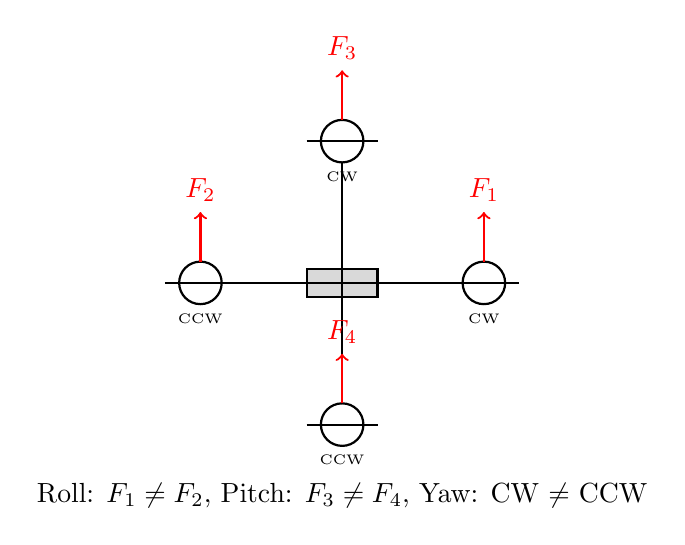
\begin{tikzpicture}[scale=0.9]
    % Body
    \draw[thick, fill=gray!30] (-0.5,-0.2) rectangle (0.5,0.2);

    % Arms
    \draw[thick] (-2,0) -- (2,0);
    \draw[thick] (0,-2) -- (0,2);

    % Motors/propellers
    \foreach \x/\y/\rot in {2/0/CW, -2/0/CCW, 0/2/CW, 0/-2/CCW} {
        \draw[thick, fill=white] (\x,\y) circle (0.3);
        \draw[thick] (\x-0.5,\y) -- (\x+0.5,\y);
        \node[font=\tiny] at (\x,\y-0.5) {\rot};
    }

    % Thrust arrows
    \draw[->, thick, red] (2,0.3) -- (2,1) node[above] {$F_1$};
    \draw[->, thick, red] (-2,0.3) -- (-2,1) node[above] {$F_2$};
    \draw[->, thick, red] (0,2.3) -- (0,3) node[above] {$F_3$};
    \draw[->, thick, red] (0,-1.7) -- (0,-1) node[above] {$F_4$};

    % Labels
    \node at (0,-3) {Roll: $F_1 \neq F_2$, Pitch: $F_3 \neq F_4$, Yaw: CW $\neq$ CCW};
\end{tikzpicture}
\caption{Quadrotor configuration showing rotor positions and control mixing.}
\label{fig:quadrotor}
\end{figure}
